\section{Concurrency}
\subsection{Khái niệm Concurrency Control}
Concurrency Control là tập hợp các kỹ thuật để đảm bảo tính đúng đắn của dữ liệu khi nhiều client truy cập và thao tác trên cùng dữ liệu cùng một lúc. Một số lỗi thường gặp bao gồm:
\begin{itemize}
    \item \textbf{Lost Update}: 2 transactions cùng ghi khiến 1 update bị mất.
    \item \textbf{Dirty Read}: Đọc dữ liệu chưa commit từ transaction khác.
    \item \textbf{Non-repeatable Read}: Đọc 2 lần ra 2 kết quả khác nhau.
\end{itemize}

\subsection{Kiến trúc 2 DBMS}
Dưới đây là bảng so sánh kiến trúc giữa MySQL và Redis:

\begin{table}[H]
\centering
\caption{So sánh kiến trúc MySQL và Redis}
\label{tab:arch-compare}
\begin{tabular}{|l|l|l|}
\hline
\textbf{Tiêu chí} & \textbf{MySQL} & \textbf{Redis} \\ \hline
Mô hình & Multi-threaded & Single-threaded \\ \hline
Cơ chế & MVCC \& Locking & Single-threaded Execution \\ \hline
Mục tiêu & Đảm bảo ACID & Đảm bảo Performance \\ \hline
\end{tabular}
\end{table}

\subsubsection{MySQL}
Mỗi connection được gán với 1 thread riêng, có thể đọc / ghi đồng thời trên cùng dữ liệu. Do đó, MySQL cần các cơ chế lock để kiểm soát truy cập:
\begin{itemize}
    \item \textbf{Shared Lock}: Cho phép nhiều transaction cùng đọc.
    \item \textbf{Exclusive Lock}: Cho phép đúng 1 transaction được đọc / ghi.
    \item \textbf{MVCC (Multi-Version Concurrency Control)}: Cho phép readers không block writers và ngược lại bằng cách duy trì nhiều phiên bản của dữ liệu. Khi tạo transaction, nó sẽ lưu trữ một Read View và chỉ có thể đọc các data ở phiên bản phù hợp.
\end{itemize}

\begin{figure}[H]
    \centering
    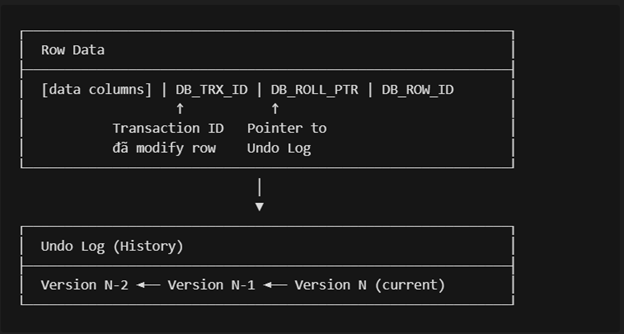
\includegraphics[width=0.85\textwidth]{figures/Kha/mvcc.png}
    \caption{Minh họa cơ chế MVCC}
    \label{fig:mvcc}
\end{figure}

\subsubsection{Redis}
Redis hoạt động Single-threaded, các transaction được xử lý tuần tự, không gặp race-condition, không phải dùng các cơ chế lock phức tạp và không bị deadlock.

\subsection{Thực nghiệm}
\subsubsection{Môi trường kiểm thử}
Các thông số môi trường thử nghiệm:

\begin{table}[H]
\centering
\caption{Thông số môi trường kiểm thử}
\label{tab:test-env}
\begin{tabular}{|l|l|}
\hline
\textbf{Thông số} & \textbf{Giá trị} \\ \hline
Cores & 8 \\ \hline
Base Clock & 3.1 GHz \\ \hline
OS & Window 11 \\ \hline
MySQL version & 8.0.x (InnoDB) \\ \hline
Redis version & Memurai (Window) \\ \hline
Dataset & Sales Transaction -- 536k transactions \\ \hline
Python & 3.13 + mysql-connector-python, redis \\ \hline
\end{tabular}
\end{table}

\subsubsection{Test đọc đồng thời}
Đo throughput khi nhiều client (thread) đọc dữ liệu ngẫu nhiên đồng thời.

\textbf{Mã nguồn Python minh họa:}
\begin{lstlisting}[language=Python, basicstyle=\ttfamily\small, breaklines=true, frame=single]
def mysql_worker_pooled(thread_id):
    conn = mysql_pool.get_connection()
    cursor = conn.cursor()
    start = time.time()
    for i in range(NUM_READS):
        tid = random.randint(1, TOTAL_TRANSACTIONS)
        cursor.execute("SELECT * FROM transactions WHERE id = %s", (tid))
        cursor.fetchall()
    elapsed = time.time() - start
    conn.close()
    return elapsed

def redis_worker_pooled(thread_id):
    r = redis.Redis(connection_pool=redis_pool)
    start = time.time()
    for i in range(NUM_READS):
        tid = random.randint(1, TOTAL_TRANSACTIONS)
        r.hgetall(f"transaction:{tid}")
    elapsed = time.time() - start
    return elapsed
\end{lstlisting}

\begin{figure}[H]
    \centering
    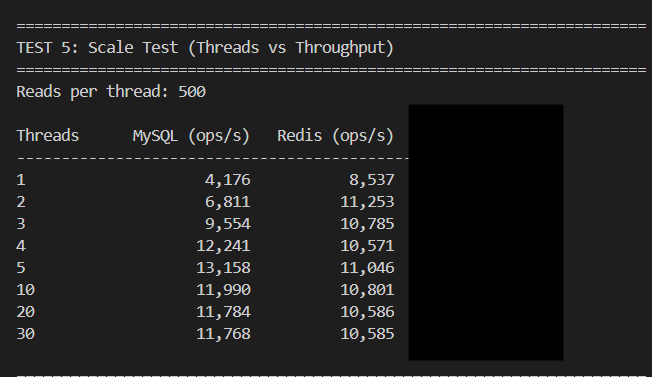
\includegraphics[width=0.85\textwidth]{figures/Kha/readtest.png}
    \caption{Kết quả test đọc đồng thời}
    \label{fig:readtest}
\end{figure}

\textbf{Nhận xét:} 
\begin{itemize}
    \item MySQL tăng trưởng theo số luồng tốt vì tận dụng multi-threading tốt. 
    \item Đến tầm 10 threads, hiệu năng MySQL bắt đầu đi ngang và giảm nhẹ do context switching và tác dụng ngược của MVCC. 
    \item Redis đạt đỉnh từ 2--5 threads và không thể tăng thêm do đơn luồng. 
    \item Khi ít thread, Redis nhanh hơn, nhưng khi nhiều thread, MySQL vượt trội hoàn toàn.
\end{itemize}

\subsubsection{Test ghi đồng thời}
Đo throughput khi nhiều client ghi dữ liệu đồng thời.

\begin{figure}[H]
    \centering
    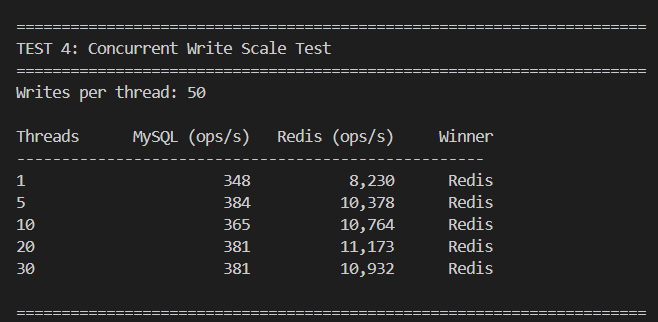
\includegraphics[width=0.85\textwidth]{figures/Kha/writetest.png}
    \caption{Kết quả test ghi đồng thời}
    \label{fig:writetest}
\end{figure}

\textbf{Nhận xét:}
\begin{itemize}
    \item Tốc độ ghi của MySQL chậm hơn Redis nhiều lần bất kể số lượng thread.
    \item \textbf{Nguyên nhân:} MySQL cần duy trì tính ACID, ghi xuống đĩa và lock dữ liệu gây bottleneck. Redis hoạt động trên RAM và không tốn chi phí tranh chấp khóa.
\end{itemize}

\subsection{Cơ chế MVCC của MySQL}

\begin{figure}[H]
    \centering
    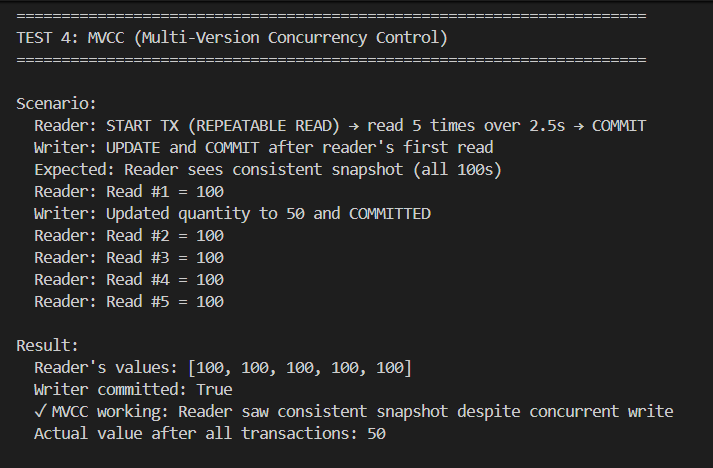
\includegraphics[width=0.85\textwidth]{figures/Kha/mvcctest.png}
    \caption{Kết quả test MVCC}
    \label{fig:mvcctest}
\end{figure}

\textbf{Nhận xét:} Reader không block Writer và ngược lại. Trong một transaction, version của một row được cố định để tránh lỗi Non-repeatable Read. Trong Redis, các lệnh chạy tuần tự nên Reader và Writer phải chờ nhau.

\subsection{Cơ chế lock trong MySQL}
MySQL sử dụng Shared Lock (S-Lock) và Exclusive Lock (X-Lock):
\begin{itemize}
    \item \textbf{Shared Lock}: Các transaction khác vẫn có thể đọc nhưng phải chờ nếu muốn ghi.
    \item \textbf{Exclusive Lock}: Không transaction nào khác được đọc hay ghi vào hàng đó.
\end{itemize}

\begin{figure}[H]
    \centering
    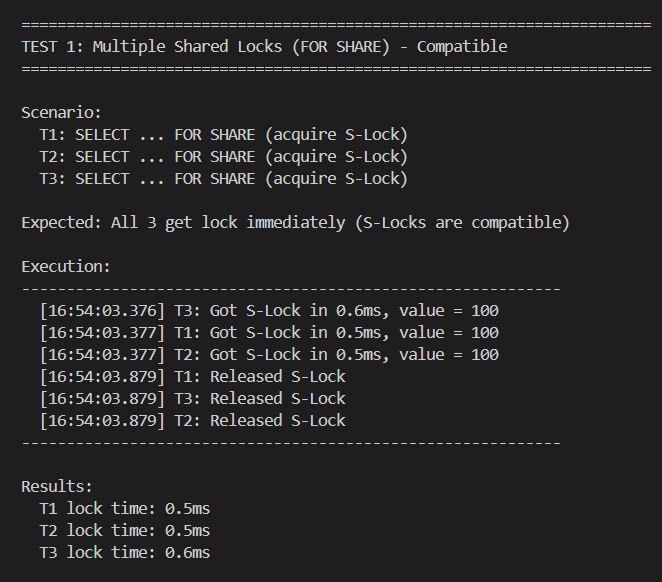
\includegraphics[width=0.85\textwidth]{figures/Kha/locktest1.png}
    \caption{Test lock -- Shared Lock cho phép đọc đồng thời}
    \label{fig:locktest1}
\end{figure}

\begin{figure}[H]
    \centering
    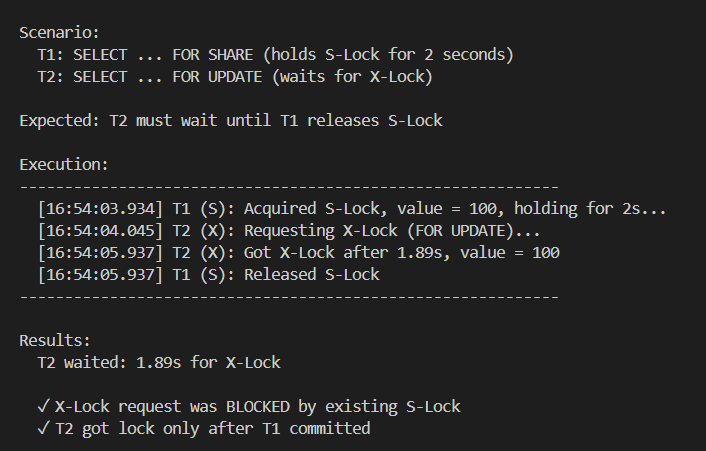
\includegraphics[width=0.85\textwidth]{figures/Kha/locktest2.png}
    \caption{Test lock -- Shared Lock chặn ghi}
    \label{fig:locktest2}
\end{figure}

\begin{figure}[H]
    \centering
    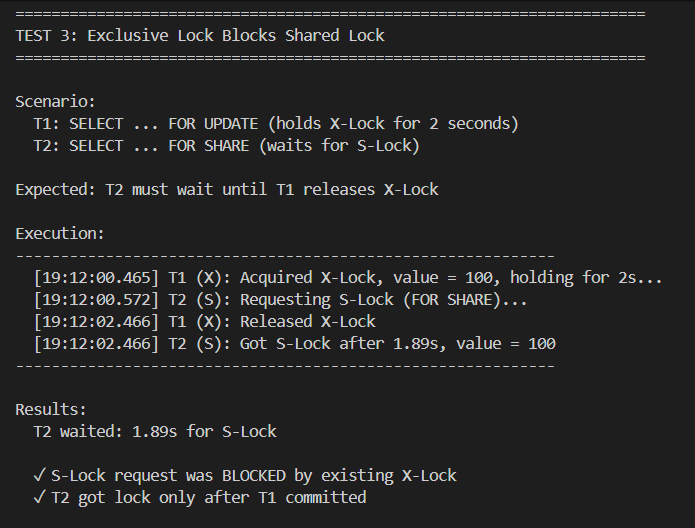
\includegraphics[width=0.85\textwidth]{figures/Kha/locktest3.png}
    \caption{Test lock -- Exclusive Lock chặn đọc và ghi}
    \label{fig:locktest3}
\end{figure}

\begin{figure}[H]
    \centering
    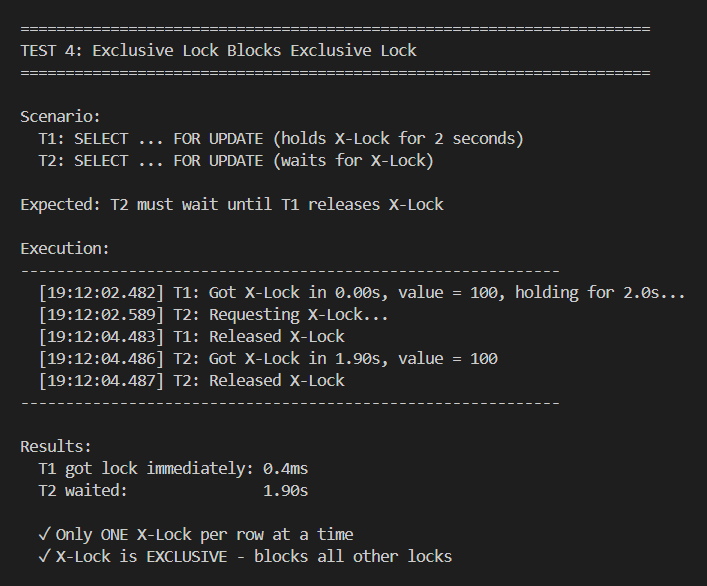
\includegraphics[width=0.85\textwidth]{figures/Kha/locktest4.png}
    \caption{Test lock -- Tổng hợp kết quả}
    \label{fig:locktest4}
\end{figure}

\subsection{Deadlock trong MySQL}
MySQL có cơ chế kiểm tra deadlock; nếu phát hiện vòng lặp chờ đợi (circular wait), nó sẽ rollback một transaction để giải tỏa nghẽn. Redis không xảy ra deadlock do kiến trúc single-threaded.

\begin{figure}[H]
    \centering
    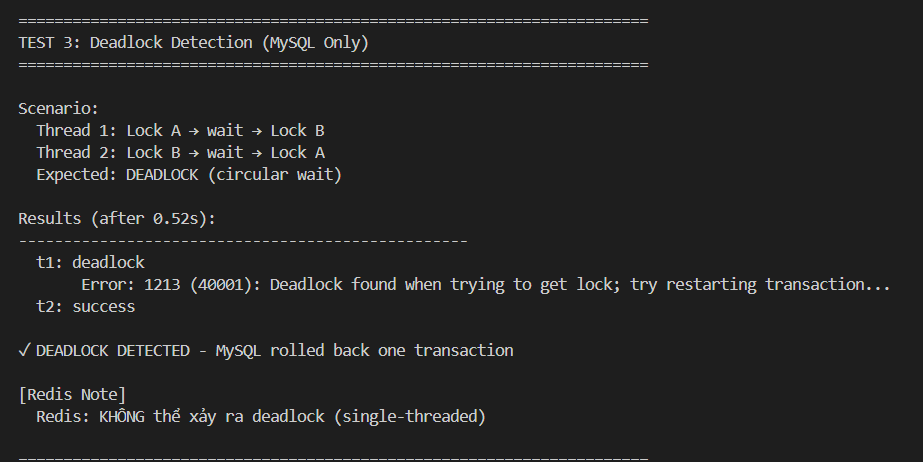
\includegraphics[width=0.85\textwidth]{figures/Kha/deadlocktest.png}
    \caption{Kết quả test Deadlock}
    \label{fig:deadlocktest}
\end{figure}

\subsection{Tính nguyên tử của Redis}
Redis chạy đơn luồng nên các lệnh đơn nguyên hoặc Lua script sẽ được xử lý tuần tự, đảm bảo tính nguyên tử (atomic) mà không cần lock.

\begin{figure}[H]
    \centering
    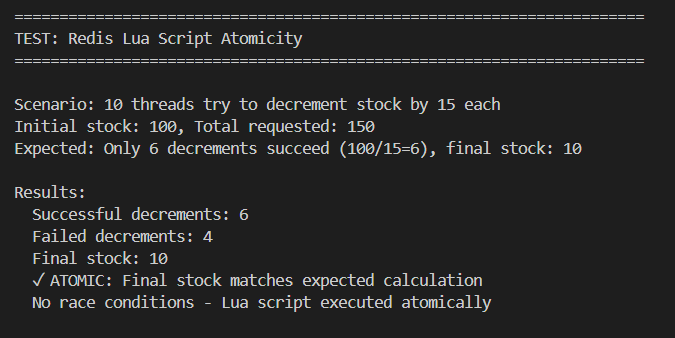
\includegraphics[width=0.85\textwidth]{figures/Kha/luaredis.png}
    \caption{Minh họa tính nguyên tử với Lua script trong Redis}
    \label{fig:luaredis}
\end{figure}

\subsection{Kết luận}
Bảng tổng kết ưu và nhược điểm của hai hệ thống:

\begin{table}[H]
\centering
\caption{So sánh ưu nhược điểm MySQL và Redis về concurrency}
\label{tab:conclusion-compare}
\begin{tabular}{|l|p{5cm}|p{5cm}|}
\hline
 & \textbf{MySQL (Multi-thread)} & \textbf{Redis (Single-thread)} \\ \hline
\textbf{Ưu điểm} & Scale với CPU cores, chạy song song query, dùng MVCC hiệu quả. & Đơn giản, tốc độ cao, không lock overhead, latency ổn định. \\ \hline
\textbf{Nhược điểm} & Phức tạp, cần quản lý lock và tune isolation level. & Bottleneck ở 1 thread, không tận dụng được đa nhân, tác vụ dài gây nghẽn. \\ \hline
\end{tabular}
\end{table}